\section{Classics}
\label{s:classics}
Works based on handcrafted pipelines are here presented.
The treatment will also focus on historical aspects of the approaches.

%%%%%%%%%%%%%%%%%%%%%%%%%%%%%%%%%%%%%%%%%
%              Hoeim
%%%%%%%%%%%%%%%%%%%%%%%%%%%%%%%%%%%%%%%%%
\subsection{Hoeim et al.}
Derek Hoeim and his collaborators produced a sequence of works on "scene interpretation" \cite{autopopup1, autopopup2, autopopup3, autopopup4, autopopup5, autopopup6}.
Only the first will be discussed in detail.

% example
\begin{figure}
	\centering
	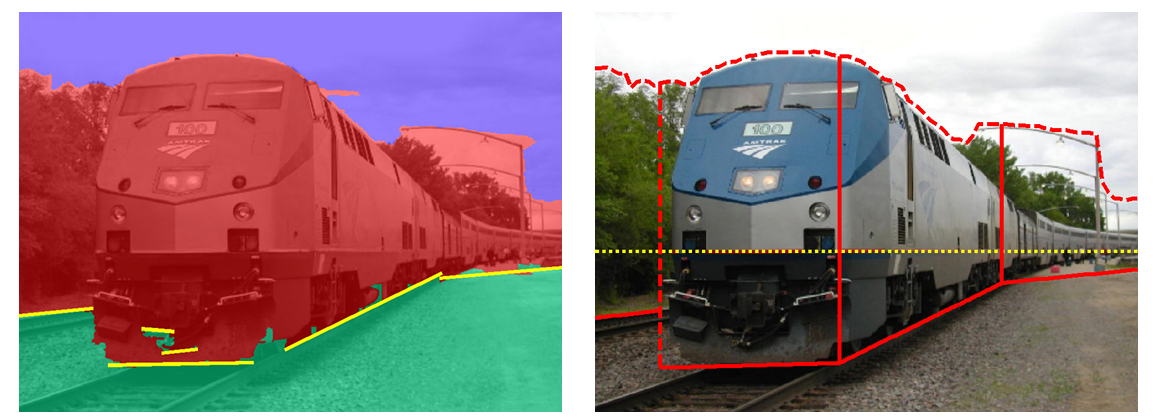
\includegraphics[scale=0.3]{figs/hoeim}
	\caption{Hoeim et al. method \cite{autopopup1}. Left: segmentation and lines fitting; Right: building the 3D model. \label{fig:hoeim}}
\end{figure}

In \cite{autopopup1} the objective is to do a simple reconstruction of the scene geometry by building a 3D model.
The reconstruction procedure is based on strong assumptions that are: the scene is composed by a ground, vertical objects stick to it and an infinite distant sky.
This obviously only work for outdoor scenes.
The ground is modeled as a plane and vertical objects as little segments of planes perpendicular to the ground and parallel to the image plane.
The pipeline is based on three phases:
\begin{enumerate}
	\item{Segmenting the image into "ground", "vertical" and "sky"}
	\item{Cleaning the segmentation}
	\item{Fitting lines to the segmented vertical regions and building the 3D model}
\end{enumerate}
In figure \ref{fig:hoeim} there is an example.
Another major assumptions is the absence of occlusion between objects.
If occlusion occurs, the segmentation procedure is not able to distinguish between different object by other means that some ground pixels in between.
Hence, in the case of occlusion, two objects at completely different depths would result in the closest to the camera.

Hoeim et al. deal with occlusion in \cite{autopopup4}, where they try to model the occlusion cues and build a computational method for occlusion detection.
The method uses a Conditional Random Field (CRF).
It was a very used statistical method in computer vision before deep learning, its main drawback is the expensive inference that involves a global optimization step.
In last years \textit{neural} CRFs have been proposed also for single image depth estimation.

In \cite{autopopup2} and \cite{autopopup5} the problem of the surface orientation prediction is tackled.
The idea, also found in older works like \cite{VideoCompass}, was to group surface normals into a predefined way.
For instance: pointing upward, pointing downward, pointing left or pointing right.
The result was a segmentation method.
At this time, for segmenting images, the main approach was to first do an over segmentation by dividing the image into super-pixels.
A super-pixels are groups of pixels that share some local property.
Second, associate to each super-pixel various numerical features, such as the histogram of colors, the number of pixels, the mean magnitude of the gradient, ...
These features were hand-crafted, in the sense that they are not learned and someone explicitly thought about them and tested them in some scenarios.
Doing so, each super-pixel has numbers associated to it.
Using a dataset of segmented images one could train a statistical learning method (e.g. a boosting method or a simple linear regression) to predict the correct labels for a given superpixel.
If the super-pixel information was not sufficient due to its locality, global optimization methods like Random Fields could have been used or iterative grouping (e.g. producing constellations of super-pixels by grouping them) was performed.

Continuing the journey of Hoeim et al., in \cite{autopopup3} the focus is on the objects.
In here object detection is tackled and the authors also attempt to orient detected objects in space.

All of these works lead to "Closing the Loop in Scene Interpretation" \cite{autopopup6} were they are all put together in a complex pipeline for building a 3D model of the scene as rich as possible.

%%%%%%%%%%%%%%%%%%%%%%%%%%%%%%%%%%%%%%%%%
%              Saxena
%%%%%%%%%%%%%%%%%%%%%%%%%%%%%%%%%%%%%%%%%
\subsection{Saxena et al.}
Saxena et al. go along the same journey and produce a series of papers \cite{saxena1, saxena2, saxena3, saxena4} which culminates in their comprehensive "Make3D: Learning 3D Scene Structure from a Single Still Image" \cite{saxena5}.
Their approach is based on Markov Random Field (MRF) models, that is a probabilistic model of the random fields family, as CRFs are.
Their idea is to over-segment the input image into super-pixels and consider them as small planar surfaces.
Planes on which super-pixels lay are modeled as 3-vectors and are the variables the MRF model has to optimize.
For defining a MRF, one has to define potential functions which define some quantity to be minimized.
In MRFs these potential functions depend on the super-pixel and its neighbours.
% example
\begin{figure}
	\centering
	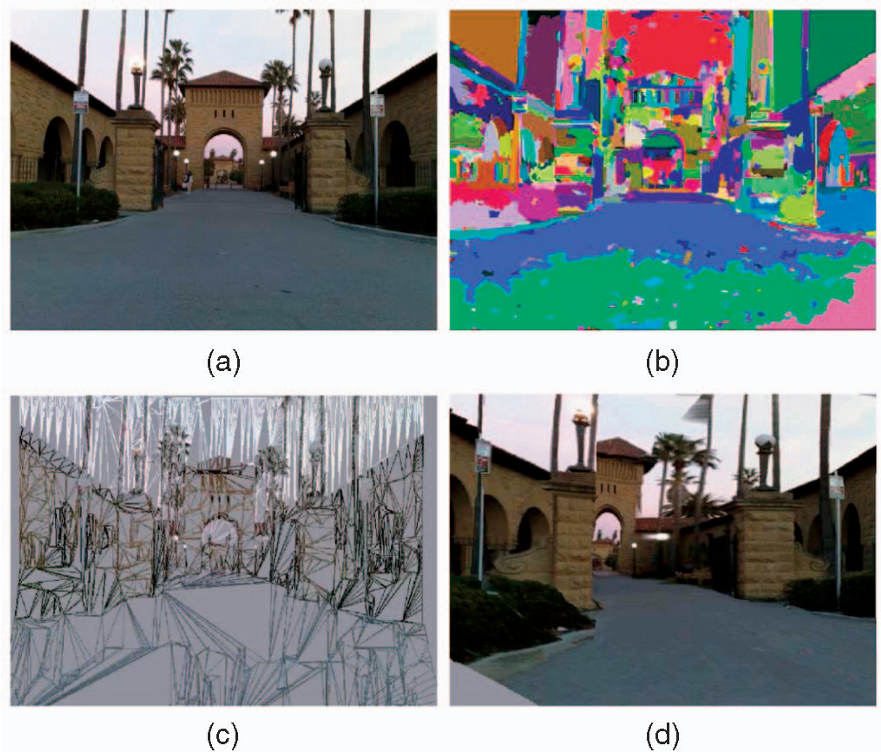
\includegraphics[scale=0.4]{figs/saxena}
	\caption{Saxena et al. example \cite{saxena5}. (a) The original image. (b) Over-segmentation of the image to obtain super-pixels. (c) The 3D model predicted by the algorithm. (d) A textured render of the 3D model. \label{fig:saxena}}
\end{figure}
Saxena et al. encode the following property in the MRF model \cite{saxena5}:
\begin{itemize}
	\item{\textbf{Image features and depth:} the content of the super-pixel is correlated to its depth;}
	\item{\textbf{Connected structure:} except in the case of occlusion, neighboring super-pixels are more likely to be connected to each other;}
	\item{\textbf{Co-planar structure:} Neighboring superpixels are more likely to belong to the same plane if they have similar features and if there are no edges between them;}
	\item{\textbf{Collinearity:} Long straight lines in the image plane are more likely to be straight lines in the 3D model.}
\end{itemize}

For training the authors gather images inside the Standford campus and create the Make3D \cite{saxena5} dataset.
It is a small dataset compared to what's available today, but at the time it was an important benchmark.

Completing their work there is a 3D model construction based on the plane parameters inferred by the MRF model.
The 3D reconstruction is based on a mesh model of the super-pixels, which can also be textured using superpixel information and as shown in figure \ref{fig:saxena}.

%%%%%%%%%%%%%%%%%%%%%%%%%%%%%%%%%%%%%%%%%
%              DepthTransfer
%%%%%%%%%%%%%%%%%%%%%%%%%%%%%%%%%%%%%%%%%
\subsection{DepthTransfer}
Karsch et al. \cite{DepthTransfer} developed DepthTransfer for tackling the monocular depth estimation problem.
Their method can be thought of as a k-NN method.
The idea is to find k-nearest neighbors in the dataset, adapt them to the current image by warping and finally stitch together parts of each of them.
The nearest neighbor search is performed by extracting a lower dimensional representation of the image and defining some distance measure in that space.
So, for instance, if in the input image appears a car, it is very likely that an image with a car is part of its k-neighbors.
By warping the retrieved image, the two cars should approximately overlap and depth values can be "transferred" to the input image (hence the name of the method).
This idea was not invented by them and can also be found in works of Konrad et al. \cite{konrad1, konrad2}.
Karsch et al. main contribution is the depth fusion process of the neighbors.
In fact, previously given various depth maps to fuse the approach was to apply some averaging function pixel-wise, for instance in \cite{konrad2} the median of the depth values is taken and a post-processing filtering is applied thereafter.
An illustration of Karsch et al. method is in figure \ref{fig:depthtransfer}
% method
\begin{figure}
	\centering
	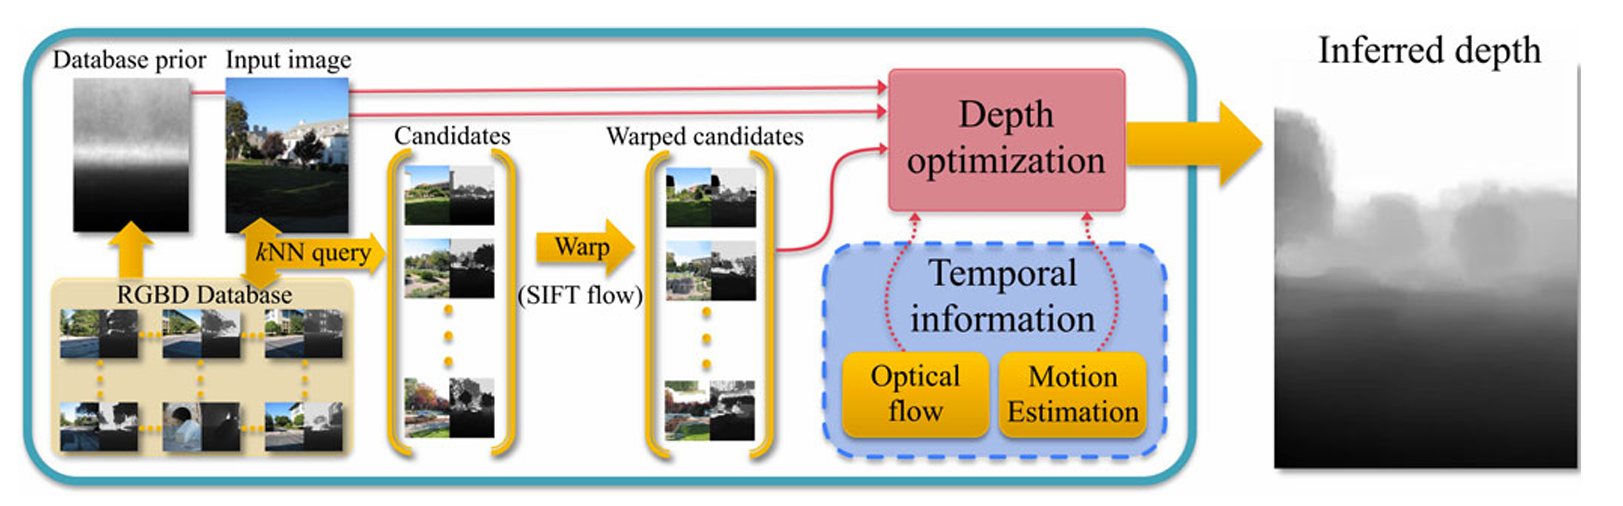
\includegraphics[scale=0.3]{figs/depthtransfer}
	\caption{Karsch et al. pipeline \cite{DepthTransfer}. The temporal information module that here appears serves the purpose to estimate depth of videos consistently predicting depth along the temporal dimension. Details are found in the paper \cite{DepthTransfer}. \label{fig:depthtransfer}}
\end{figure}

Before fusing the depth maps a preliminary warping is applied.
The warping is computed through SIFT Flow procedure \cite{SIFTFlow} that computes SIFT features pixel-wise and create a bijection between the pixels of the two images based on the computed features.
It is an expensive procedure though and today it could be substituted by some Optical Flow neural model.
After the warping is performed, the fusion is performed through a global optimization procedure which (simplifying) pixel-wise chooses from which image to take the depth value from.

%%%%%%%%%%%%%%%%%%%%%%%%%%%%%%%%%%%%%%%%%
%              IM2CAD
%%%%%%%%%%%%%%%%%%%%%%%%%%%%%%%%%%%%%%%%%
\subsection{IM2CAD}
This work is from Izadinia et al. \cite{IM2CAD} and it is the direct evolution of the work from Lawrence Robert, whose quote starts the chapter.
Unlike the other papers discussed in this section, this uses deep learning and is relatively recent (2017).
Nevertheless, its ideas are rooted in the work of Lawrence Robert P.h.D. thesis, dated 1963.
Let's start immediately by looking at a representation of their inference pipeline in figure \ref{fig:im2cad}

% method
\begin{figure}
	\centering
	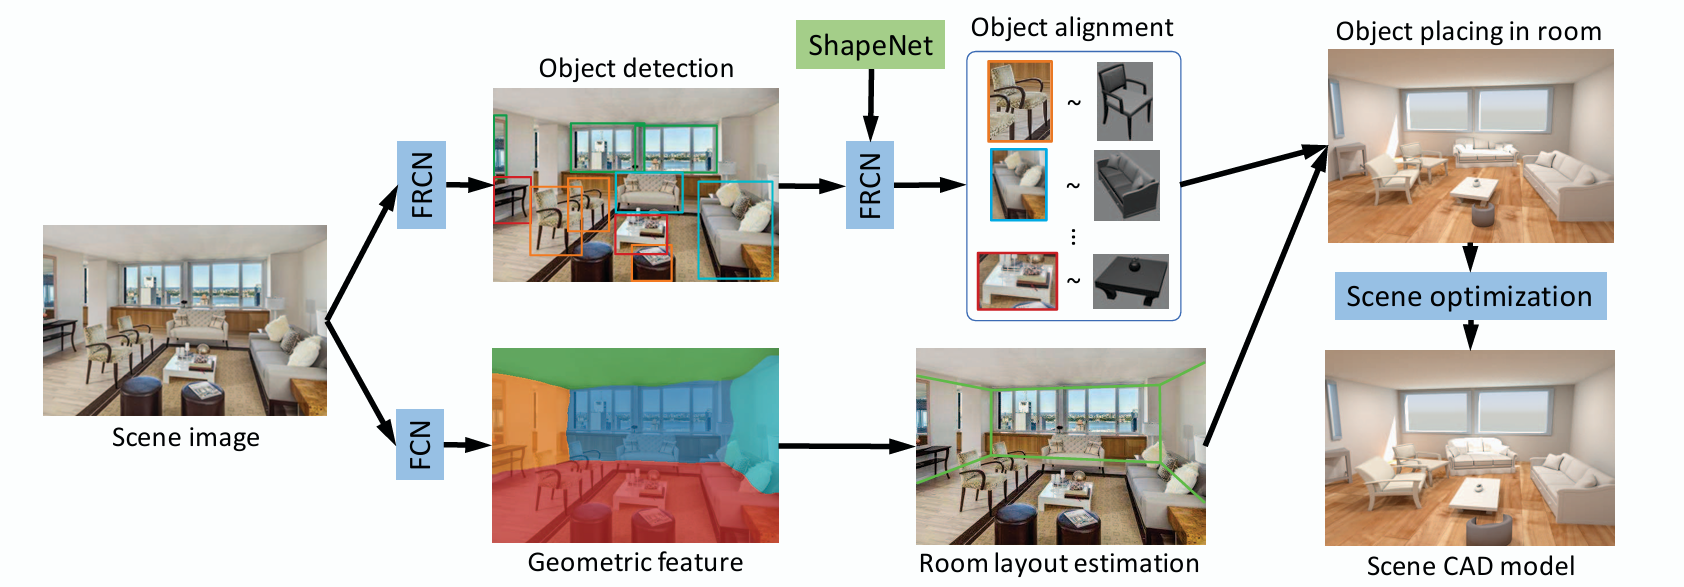
\includegraphics[scale=0.3]{figs/im2cad}
	\caption{Izadinia et al. \cite{IM2CAD} pipeline. \label{fig:im2cad}}
\end{figure}

First, it must be said that this method works exclusively in indoor environment that resemble the appearance of a "house room".
Similarly to what Hoeim et al. did in their method, here objects and background are treated separately.
There is a neural object detector that deals with furniture filling up the room and a neural segmentation model that subdivide the pixels into 5 categories corresponding to the 3 walls, the ceiling and the floor that a person can see by standing in a room.
This implies another limitation of the method: the room must have exactly 4 walls.
Now, a neural network compares the object detected with a CAD dataset of object appearances and match the detection with some real world 3D model of furniture by aligning its orientation in space.
Contemporary room layout estimation method builds a simple 3D model of the room.
Objects and room are now known.
The final step is to optimize the information found.
In order to do so, 3D models are placed in the room based on the initial guess given by the alignment procedure.
The 3D model is textured and rendered (illumination is given by windows and lights found in the room).
An iterative process compares the rendered view with the input image and adjusts the orientation, size and location of the objects until a criterion is fulfilled.
Eventually the scene CAD model is returned.

\section{Deep Learning and Interpretability}
\label{sec:deep learning and interpretability}
Since the advent of machine learning (ML) and artificial intelligence (AI), there has been a paradigm shift in solving problems in a lot of fields.
Instead of designing an algorithm that directly solves a given task, a learner is delegated to find a good-enough solution in a pool of possible solutions by solving an optimization problem defined on a set of data points \cite{ML_book}.
Among all, deep learning (DL) techniques are the most successful ones and have a much superior performance than the statistical learning counterparts in the most challenging tasks (vision, language, autonomous agents, …), provided data is enough.
Deep learning is more scalable w.r.t. dataset size and data dimensionality than statistical learning techniques are and is better suited for exploiting the existing hardware, which in turn was improved for the purpose during last years.
This made DL solutions successful, popular and spreading to more and more research fields, supported by an ever-growing data and hardware availability \cite{DL_overview}.

Although deep learning models are very effective, it is very difficult for a human (experts included) to understand how these models come up with their outputs due to their large sizes, the (general) high-dimensionality of their inputs and training algorithms.
For they are considered black boxes \cite{DL_overview}.
Indeed, humans understand which mathematical operations DL models carry out in order to compute numerical outputs, but they are not capable of intuitively interpreting those computations so that they represent something meaningful for them.
But why should humans be interested in understanding these models? 
If a model has been experimentally proven to be reliable, it is not involved in critical scenarios or, it has a limited impact on people and things, then not understanding its functioning doesn't raise concerns.
Yet, there are a lot of applicative contexts in which this is relevant, e.g. autonomous driving \cite{Zablocki2022}, Industry 4.0 \cite{XAI_industry} and healthcare \cite{XAI_healthcare}.
More generally, when the formal numerical objectives and metrics of a learning algorithm are not rich enough to describe real-world deployment settings, the need for a more thorough understanding arises \cite{Lipton}.
This, combined with the integration of AI in everyday life, results in society, ethics and legislation demanding a new generation of AI whose functioning is more transparent.
This trend is also observed in the rising number of publications during the last decade \cite{XAI_review} in the field of "eXplainable" Artificial Intelligence (XAI) which addresses this exact matter, particularly in relation to ML and DL.

The main property of an AI system studied by this field is its \textit{interpretability}.
This term is not rigorously defined since each author gives his/her own specific definition \cite{XAI_review}.
For example Miller \cite{Miller} defines interpretability as the degree to which humans can understand the cause of a decision made by an artificial intelligent system (its numerical output). 
While, Kim et al. \cite{examples_enough} give a more operative definition of interpretability as the capacity of humans to correctly and efficiently predict the AI system results, yet a lot of other definitions and characterizations have been proposed, e.g. see \cite{Lipton}.
Without limiting the discussion to a precise definition, interpretability can be thought as an intuitive understandability of an AI system and the way it produces predictions.
XAI addresses the problem of developing methods for generating explanations accounting for such predictions (post-hoc methods) or design principles to build systems intrinsically more interpretable (ante-hoc methods).

There exist some intrinsically interpretable models such as sparse linear regression, shallow decision trees or K-nearest neighbors \cite{molnar2022} \cite{XAI_review}.
Their limited size and mathematical complexity are easily understandable by a human expert but suffer from low accuracy, especially when tackling complex tasks.
In fact, a general trade-off between accuracy and transparency is known to exist in AI.
An algorithm is said to be transparent if it is understandable by a human without the use of explainability techniques.
XAI studies models that traded off transparency for high accuracy by developing methods for clarifying their behavior after training has been performed (post-hoc interpretability methods), or aims at designing models that try to alleviate the limitations of that trade-off in advance (ante-hoc interpretability methods), for instance by being trained to return both a prediction and an explanation for it. 

There are other criteria for classifying interpretability criteria \cite{molnar2022}.
Distinctions can be made based on what kind of result an interpretability method returns.
For example there are methods that return counterfactual explanations for justifying a prediction.
If the model $f$ on the input $x$ returned the output $y = f(x)$, a counterfactual explanation would be an input $x'$ close to $x$ such that $f(x') = y' \neq y$ \cite{Zablocki2022}.
This explanation attempts to answer the question “What should have happened instead of $x$ so that $y'$ occurred?” by either finding $x'$ in the training dataset or by generating it trough generative AI techniques \cite{Zablocki2022}.
Some methods return a natural language explanation, this is the case for Xu et al. \cite{9157111} who developed a DL model for an autonomous driving toy setting producing both an output and a natural language explanation for it.
This was made possible thanks to annotated examples in the dataset employed. 

Another distinction can be drawn between so-called model-specific and model-agnostic methods \cite{molnar2022}.
Some interpretability methods are developed for a specific family of ML or DL models (e.g. Deconvnet \cite{Deconvnet}) leveraging on their specific mathematical structure and are thus named model-specific methods.
Other methods treat the model as a black box to probe, trying to model its behavior in a simpler way, an example of this is LIME \cite{LIME} which tries to locally linearly approximate the model by fitting a sparse linear regression model.
The fitted transparent model constitutes the explanation.

Finally, interpretability methods can be classified as local or global.
Local methods address interpretability of a single prediction of the studied AI model (i.e. around a single data point $x$), while global methods take into account the overall model behavior.
The above-mentioned methods are local.
A global method can consist in a feature selection procedure for identifying a subset of the input features that have more predictive power w.r.t. the others \cite{molnar2022}.
Global methods are more common in ML methods rather than DL ones. 

Lipton \cite{Lipton} identifies five aspects of an ML model on which XAI can shed light on.
These are:
\begin{itemize}
\item{\textbf{Trust}: If confidence that the model properly performs in real-world scenarios is 
required and numerical assessments of its performance are not sufficiently 
expressive, then trust has to be built in other ways, a more deep understanding of 
the model helps in this direction. Trust is especially needed in critical applications 
like in medical decision-making \cite{XAI_healthcare} and autonomous driving \cite{Zablocki2022}, where extensive 
testing is difficult to achieve due to safety, economical or legal concerns.}
\item{\textbf{Causality}:
Especially in scientific research, where ML models are a way to extract information about the world, relations inferred by the these methods are not guaranteed to reflect real causal relationships.
By understanding the fitted models scientists could gain new insights and test them through new experiments.
}
\item{\textbf{Transferability}:
It is common that training settings do not match deployment environments due to their complexity or non stationarity.
Robustness to changes is a desirable property in this case and particularly desired in industrial settings \cite{XAI_industry}. 
Understanding the AI model can serve the purpose of inspecting how suitable it is for deployment.
}
\item{\textbf{Informativeness}:
Even though understanding an artificial intelligence model is sometimes very difficult (in particular neural networks), trying to do it can nevertheless convey useful information.
For instance, an explanation to the output of a diagnosis model can highlight clinical details missed by a doctor \cite{XAI_healthcare}.
}
\item{\textbf{Fair and Ethical decision-making}:
Since ML models learn from data and data reflect society biases, these are likely to be biased as well.
For example this happens for language models, algorithms for recruitment or for granting loans. 
Only a thorough investigation of the AI system functioning is able to reveal these biases.
}
\end{itemize}
By inspecting an AI model with the above-mentioned interpretability techniques, a human can acknowledge the presence or absence of properties related to these five aspects.

\section{Single Image Depth Estimation and Interpretability}
\label{sec:SIDE and interpretability}
There are a lot of works about interpretability of neural networks for vision, but the most studied tasks are image classification, object detection and image generation.
Despite the growing interest for monocular depth estimation, driven also by its relevance in robotics and autonomous driving applications, its interpretability side is yet to be deepened.
I will review here three relevant works on interpretability of single image depth estimation models that tackles the problem from different perspective:
\begin{itemize}
    \item{Dijk et al. \cite{Dijk} probe neural depth estimators in search for correlation with human visual cues;}
    \item{Hu et al. \cite{Hu} develop a (neural) method for visualizing relevant pixels for the estimation process;}
    \item{You et al. \cite{towards_interpretable} formulate a regularization term aiming at both measuring and increasing interpretability of the models.}
\end{itemize}

\subsection{Dijk et al.}
Depth perceptions in humans has been widely studied.
Human visual depth cues associated with full scene understanding by humans are divided into primary cues and secondary ones \cite{monocular2024}.
The primary cues, as reported in \cite{monocular2024}, are:
\begin{itemize}
    \item{
        \textit{Relative size} refers to the apparent difference in the area occupied by the projection of objects of physically similar size on the retina.
        In other words, between two similar objects, the one that seems smaller is farther from the observer.
    }
    \item{
        \textit{Relative density} is detected when there is a cluster of similar objects or textures.
        As the distance from the observer increases, the objects appear to be closer to each other and the textures become denser.
    }
    \item{
        \textit{Height in the visual field} is connected with the relation of the bases of objects, assuming the presence of a ground plane and the absence of a ceiling.
        Specifically, objects at a greater distance from the observer tend to appear closer to the horizon line.
    }
    \item{
        \textit{Aerial perspective}  appears when the air has a high concentration of moisture, pollution, or both, and the objects in the distance become bluer, have less contrast, or both in comparison to those in the foreground.
    }
    \item{
        \textit{Motion Perspective} is the phenomenon that appears when there is relative motion between the observer and observed objects.
        Objects that appear to be moving faster are closer to the observer.
    }
    \item{
        \textit{Convergence} is connected with the angle between the optical axes of the two eyes.
        If an object is far from the observer, the optical axes tend to be parallel and the angle between them is close to zero degrees.
        As the object distance decreases, the two axes converge to a point on the object.
    }
    \item{
        \textit{Accommodation} is the eye function in which the lens (which is essentially an asymmetric biconvex lens) changes its shape to enable focusing at different distances.
    }
    \item{
        \textit{Binocular Disparity} the bases for what is called stereo vision, is the difference in the location of an observed object in the two eyes and only has meaning if more than one viewing sensors (eyes in this case) are available.
    }
\end{itemize}
Secondary cues are instead texture gradients, linear perspective, brightness and shading, kinetic depth, kinetic occlusion, and gravity.
These cues are “secondary” because they are either a combination of the main or they are incorrectly taken into account.
Secondary cues are particularly relevant for monocular depth estimation since the primary cues mainly rely on both of the eyes.
An illustration of some of these cues can be found in figure \ref{fig:cues}.

% human depth cues
\begin{figure}
    \centering
    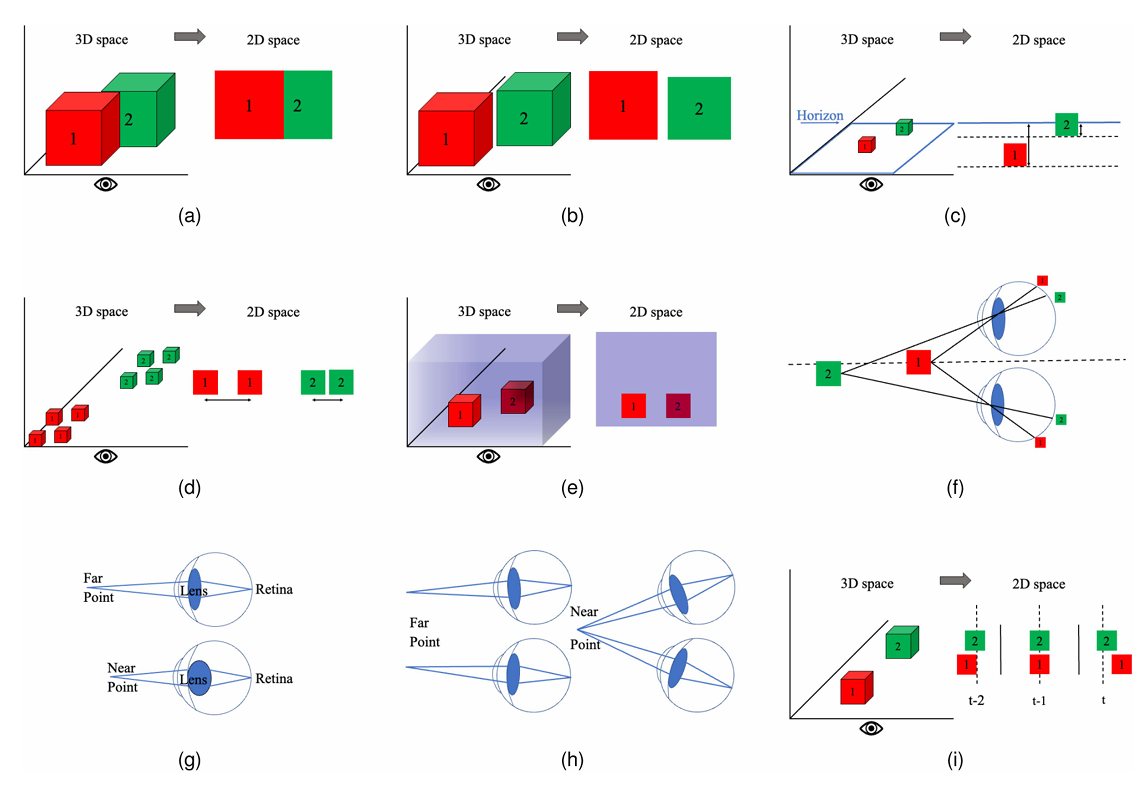
\includegraphics[width=1.\textwidth]{figs/cues}
    \caption{
        Image from \cite{monocular2024}. Visual depth cues: (a) occlusion, (b) relative size, (c) height in the visual field, (d) relative density, (e) aerial perspective, (f) binocular disparity, (g) accommodation, (h) convergence, and (i) motion perspective.
        In cases (a)-(e) and (i) left side is the 3D representation of two objects and the right side is the corresponding 2D projection attained by a monocular observer.
        \label{fig:cues}
    }
\end{figure}

In \cite{Dijk}, Dijk et al. investigate the use of apparent size of objects and their position in the image by neural model estimating depth from single image.
They focus only on these cues since they argue that in the KITTI dataset, which is their test ground, the others are not relevant.
For instance, aerial perspective is not observed in KITTI images due to relatively low depth values while on a dataset like Cityscapes it is an observable atmospheric effect.

Given an image depicting an object of well known size and lying on the ground, it is possible to estimate its depth from its apparent size or its position w.r.t. the horizon.
Camera pose and parameters must be known to this extent.
In the first case, the object apparent size is inversely proportional to its depth, while in the second case the higher the object appears in the image (i.e. closer to the horizon line), the farther it is.
Depth values estimated in these two ways do not necessarily coincide.

\begin{figure}
    \centering
    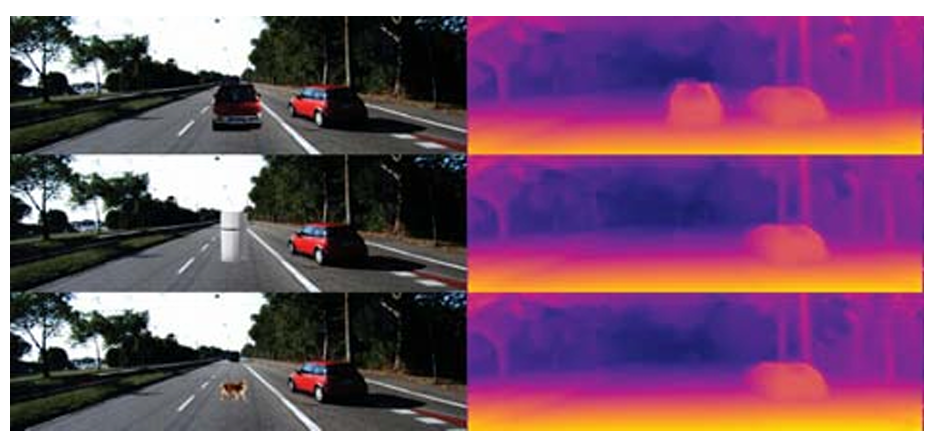
\includegraphics[width=1.\textwidth]{figs/object_disappearing}
    \caption{
        Image from \cite{Dijk}.
        Objects that are not found in the training set are not reliably detected if hard-pasted into the image.
        \label{fig:object_disappearing}
    }
\end{figure}

The authors of the papers use this fact to probe the network and measure the variation in depth across a set of hand-crafted examples.
They put a car of fixed size in different points of the image, corresponding to different depth points in real-world, and also put the same care in a fixed spot but varying its size.
What Dijk et al. observe is that neural networks rely primarily on the vertical position of objects rather than their apparent size \cite{Dijk}.
This is due to the fact that the depth of the manually inserted car was independent on its size, but it seemed to be completely determined by its vertical position.

The use of vertical position as a depth cue implies that the considered networks have some knowledge of the camera pose.
Since the KITTI dataset exhibits an approximately constant camera pose (except for some frame where the recording car bumps into some sloped terrain), a natural question is whether the network assumes the camera pose constant or it estimates it image-wise.

Again, the authors design some experiments that show something in between: the camera pose is generally under-estimated when either a pitch or a roll in the camera happens.


\begin{figure}
    \centering
    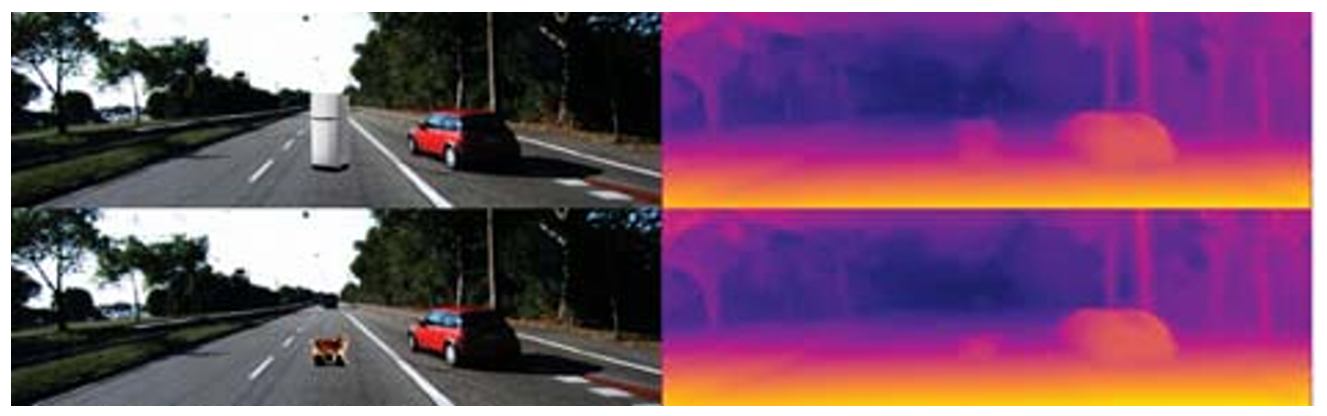
\includegraphics[width=1.\textwidth]{figs/object_appearing}
    \caption{
        Image from \cite{Dijk}.
        A shadow is added to the bottom of the objects.
        They are detected, although their shape is not properly recognized.
        \label{fig:object_appearing}
    }
\end{figure}

The last matter Dijk et al. investigate is object recognition.
A first focus is put onto color and texture and, by passing to the networks images with altered coloring and/or textures, they observed that depth estimation models seem to be invariant to image coloring as long as texture is preserved.
More interestingly, they studied how the networks detect obstacles.
They observed the following strong bias of models trained on the KITTI dataset: objects that cast a strong dark shadow on the ground are detected and their depth is given by the position of their shadow (coherently with what observed in the experiments on depth cues).
In figure \ref{fig:object_disappearing} it can be seen that the presence of new objects is completely ignored in the respective depth map.
Instead, in figure \ref{fig:object_disappearing}, after the adding of theirs shadows, the considered objects appear in the depth map.

\subsection{Hu et al.}
Hu et al. \cite{Hu} investigate single image depth estimation models by attempting to visualize which pixels were relevant for the prediction.
As they point out, there are popular and arguably useful methods for producing visual explanations of image classification models predictions such as CAM \cite{CAM} and GradCAM \cite{GradCAM}, but they cannot be directly applied to CNNs performing depth estimation.
This holds true also for other explainability methods.

Thus, the authors employ another approach for visualization.
They formulate the problem of identifying relevant pixels as a problem of sparse optimization \cite{Hu}.
The underlying assumption made in this work is that  CNNs can infer depth map equally well from a properly selected subset of pixels of the input image.
Let's call $\mathbf{I}$ the input RGB image tensor of shape $H \times W \times 3$, $f_{pred}$ is the network and $\mathbf{Z} = f_{pred} ( \mathbf{I} )$ is the predicted depth map.
The objective is to specify a mask $\mathbf{M}$, that is a binary tensor of shape $H \times W \times 1$ that specifies which pixels are important in the image.
$\mathbf{M}(p) = 1$ means that $p$ is relevant for predicting the depth on that image, $\mathbf{M}(p) = 0$ otherwise.
By "relevant", Hu et al. mean that $f_{pred} (\mathbf{I}) \approx f_{pred} (\mathbf{I} \, \odot \, \mathbf{M})$, where $\mathbf{I} \, \odot \, \mathbf{M}$ is performed by tensor broadcasting.
Other works tried this same approach for producing useful relevant-pixels visualization for other computer vision tasks.
The main problem is how to find a suitable mask that is meaningful to humans.
Regularization terms constraining the mask can be specified for achieving this, but the choice here is to produce the mask through another neural network, constraining it to a certain manifold specified by the new model.

\begin{figure}
    \centering
    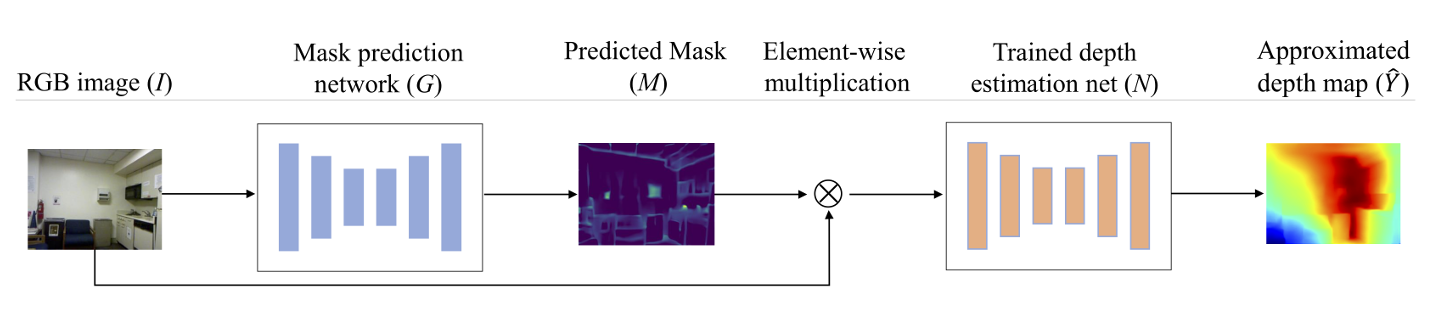
\includegraphics[width=1.\textwidth]{figs/hu}
    \caption{
        Masking method from \cite{Hu}.
        Notation is different: $G$ corresponds to $f_{mask}$, $N$ to $f_{pred}$ and $\hat{Y}$ to $\hat{\mathbf{Z}}$.
        \label{fig:hu}
    }
\end{figure}

Let's call $f_{mask}$ the neural network that takes as input the image $\mathbf{I}$ and outputs the mask, formally $\mathbf{M} = f_{mask}(\mathbf{I})$.
A representation of the pipeline can be found in figure \ref{fig:hu}.
For making things differentiable, the mask is treated as a continuous object with values in $[0, 1]$.
The continuous masks will be thresholded during the visualization phase.
The network $f_{pred}$ is frozen during the training of network $f_{mask}$ and the loss function used is:
\[
    \mathcal{L}_{dif} (\mathbf{Z}, \, \hat{\mathbf{Z}}) +
    \lambda \frac{1}{HW} \big\| \mathbf{M} \big\|_{1}
\]
Where $\hat{\mathbf{Z}} = f_{pred}(\mathbf{I} \, \odot \, \mathbf{M})$, $\lambda$ a hyperparameter and $\mathcal{L}_{dif}$ is a measure of difference between the two predicted depth map.

By visually investigating the obtained masks, Hu et al. discover that the mask tend to be similar to the edge map of the image.
Though there are differences.
First: not all edges are relevant for depth estimation, it can be seen in the first image of the figure \ref{fig:pixel_relevance} that edges corresponding to white striped on the street are masked out.
Second: masks tend to be "thicker" than edge maps, in the sense that there are some filled regions.
In the case of the KITTI dataset (as depicted in the figure \ref{fig:pixel_relevance}), the region corresponding to the vanishing points of the scene seem to be particularly important for the model considered.
The authors performed various experiment also on the NYU-v2 dataset and by varying the hyperparameter $\lambda$ which controls the sparseness of the mask.

\begin{figure}
    \centering
    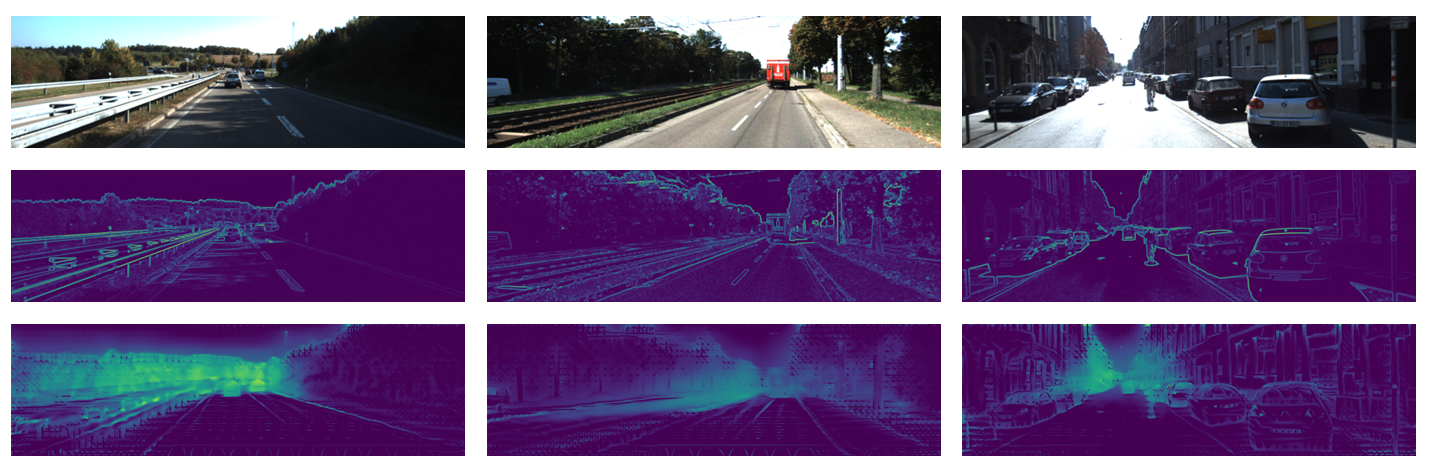
\includegraphics[width=1.\textwidth]{figs/pixel_relevance}
    \caption{
        Masks from \cite{Hu}.
        Top row: original images from KITTI.
        Middle row: edge maps.
        Bottom row: predicted masks.
        \label{fig:pixel_relevance}
    }
\end{figure}

\subsection{You et al.}
A more recent work is that of You et al. \cite{towards_interpretable}\footnote{With a title ("Towards Interpretable Deep Networks for Monocular Depth Estimation") very similar to the one of my thesis...}.
In their work they try to quantify the interpretability of neural networks for monocular depth estimation by measuring depth selectivity of their units.
They also propose a regularization term for training such networks that enhance their interpretability, as defined by them, and do not harm performance.

The main idea is to measure the depth selectivity of deep feature maps channels.
Namely, the tendency of a channel to have high activation in correspondence of pixels associated to a specified depth range.

Formally, consider an input image $\mathbf{I}$, the ground truth depth map $\mathbf{Z}^{*}$ and the intermediate feature maps $\mathbf{F}_{l}$ labeled by the respective layer $l$.
Each feature map tensor has shape $H_{l} \times W_{l} \times C_{l}$, as $l$ increases (i.e. deeper feature maps are considered) $H_{l}$ and $W_{l}$ decrease and $C_{l}$ increases.
You et al. consider the "response" $R_{l, c}^{b}$ of a certain channel $c$ at a certain depth $l$ w.r.t. a depth range $b$.
In order to do so, first the depth range is divided into $B$ (uniform) bins.
Second, given a certain input-output pair $(\mathbf{I}, \, \mathbf{Z}^{*})$ a mask that identifies which pixels fall into the $b$th-bin is defined:
\[
    \mathbf{M}_{b}(i, \, j) \, = \, \begin{cases}
        1 & \text{ if } \mathbf{Z}^{*}(i, \, j) \in b \text{th-bin} \\
        0 & \text{ otherwise}
    \end{cases}
\]
Now, to get the response $R_{l, c}^{b}$ of the channel $c$ at depth $l$ with respect to the depth range $b$, the $c$th-channel of the feature map $\mathbf{F}_{l}$ is averaged by weighting it with the computed mask $\mathbf{M}_{b}$.
Before computing such a weighted average, the $c$th-channel of the feature map $\mathbf{F}_{l}$, of shape $H_{l} \times W_{l}$, is up-sampled to $\mathbf{F}_{l, c}^{\uparrow}$ of shape $H \times W$.
The response is averaged across the whole dataset to get the final response $R_{l, c}^{b}$.
\begin{figure}
    \centering
    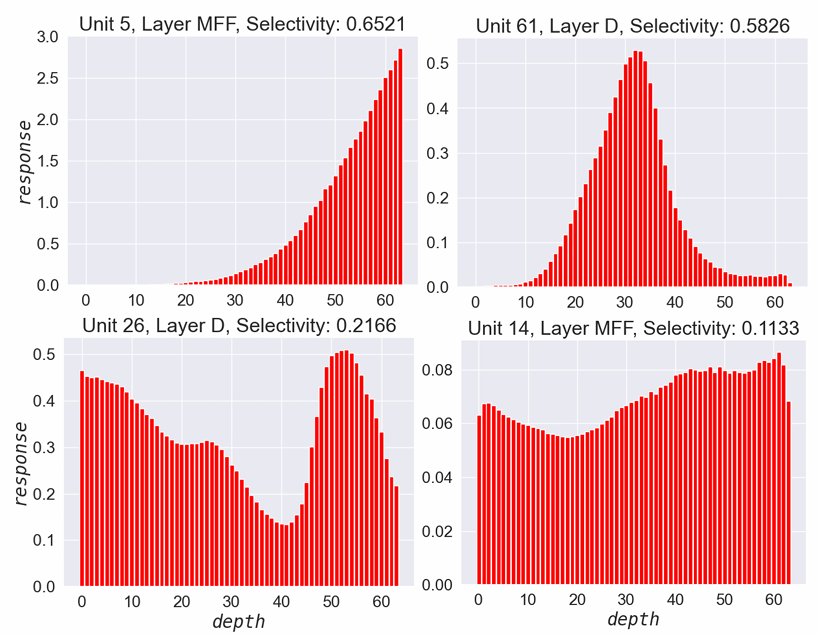
\includegraphics[width=0.6\textwidth]{figs/selectivity}
    \caption{
        Depth selectivity of a trained neural network for depth estimation.
        Histograms of $R_{l,c}^{b}$ for certain channels (called "units" in the picture) and layers (MFF and D are the names of the layers in the considered architecture) from \cite{towards_interpretable}.
        Depth was discretized into 64 bins as can be observed from the horizontal axis.
        Selectivity of each channel-layer pair is also reported.
        Some channels exhibit depth selectivity (top row), while in others it completely misses (bottom row).
        \label{fig:selectivity}
    }
\end{figure}

Hence, a response is a number. The higher the number and the more probable it is for neurons at channel $c$ at depth $l$ to fire in correspondence of pixels of depth in the $b$th bin.
A channel is depth selective if it fires only w.r.t. a certain depth bin.
To quantitatively measure the depth selectivity of a channel $c$ at depth $l$, $DS_{l, c}$, the authors use a formula that comes from neuroscience \cite{towards_interpretable}.
Some preliminary definitions:
\[
    R_{l, c}^{max} = \text{max}_{b \in [B]} R_{l, c}^{b}
\]\[
    \bar{R}_{l, c}^{-max} = \text{mean}_{R_{l, c}^{b} \neq \, R_{l, c}^{max}} \, R_{l, c}^{b}
\]
Thus the depth selectivity is defined as:
\[
    DS_{l, c} = \frac
        {|R_{l, c}^{max}| - |\bar{R}_{l, c}^{-max}|}
        {|R_{l, c}^{max}| + |\bar{R}_{l, c}^{-max}|}
\]

$DS_{l, c}$ ranges in $[0, 1]$ and the higher, the more selective channel $c$ in layer $l$ is.
The authors measure the responses of some relevant layers of a pre-trained model for depth estimation.
A graph can be seen in figure \ref{fig:selectivity}.
The mean depth selectivity of the model from which the responses were measured is 0.46.
The mean depth selectivity of a random assignment of depths is 0.3, hence there is some minimal depth selectivity also in models trained without additional constraints.

\begin{figure}
    \centering
    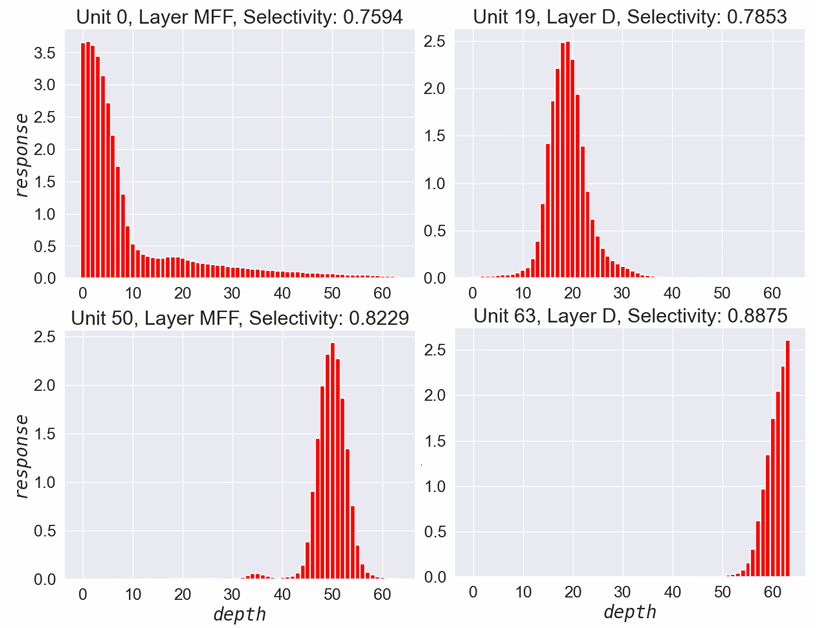
\includegraphics[width=0.8\textwidth]{figs/increased_selectivity}
    \caption{
        The content is analogous to that of the figure \ref{fig:selectivity}, but it refers to a model regularized with the introduced term.
        The depth selectivity of the considered channel-layer pairs is evident.
        \label{fig:increased_selectivity}
    }
\end{figure}

With the purpose of making depth estimation models more interpretable, You et al. propose a regularization term to be used during training.
The authors discard a simpler approach (that is: to directly increase general depth selectivity during training) in favor of a more stable formula.
After assigning to each channel $c$ of a certain layer $l$ of the feature map a bin $b_{c}$, they define the following:
\[
    \bar{R}_{l, c}^{-b_{c}} = \text{mean}_{b \neq b_{c}} R_{l, c}^{b}
\]
The assignment of bins to channels consists of a simple heuristic: given $C_{l}$ channels and $B$ bins, arbitrarily assign $C_{l} / B$ to each bin.
$B$ is chosen so to divide $C_{l}$.
Finally, the regularization term is given by:
\[
    \mathcal{L}_{reg} =
    \sum_{l \in L} \,
    \sum_{c \in [C_{l}]} \,
        \frac
            {|R_{l, c}^{b_{c}}| - |\bar{R}_{l, c}^{-b_{c}}|}
            {|R_{l, c}^{b_{c}}| + |\bar{R}_{l, c}^{-b_{c}}|}
\]
Where $L$ is the set of layers to which apply the regularization.
After training the network using this additional term, You et al. observe an increase in the depth selectivity of the model both globally, with a mean depth selectivity of 0.83, and also locally.
Comparing the figure \ref{fig:increased_selectivity}  with \ref{fig:selectivity}, it can be seen how the histogram of responses peaks more, implying a higher depth selectivity for that channel-layer pair.